\documentclass{article}

\usepackage[T1]{fontenc}    %Schriftart des Dokumentes
\usepackage[ngerman]{babel} %Dokumentensprache, hier Deutsch
\usepackage{amsmath, amssymb, stmaryrd} %mathematische Schriftzeichen
\usepackage{graphicx} %Einfügen von Grafiken
\usepackage{wrapfig}
\usepackage{bm}
\usepackage{array}
\newcommand\rowincludegraphics[2][]{\raisebox{-0.45\height}{\includegraphics[#1]{#2}}}

\setlength{\parindent}{0pt} %Einrückung von Absätzen auf null gesetzt
\setlength{\parskip}{10pt} %Abstand zischen Absätzen auf 10pt gesetzt

\title{Versuch 25: Oszilloskop}
\author{Matthias Kuntz}
\date{02.10.2023}

\begin{document}

\maketitle

%-------------------------EINLEITUNG-------------------------
\section{Einleitung}

Dieser Versuch dient nicht direkt dem bestimmen von Naturkonstanten oder der Untersuchung eines physikalischen Phänomens. Vielmehr dient er dem Kennenlernen der Funktionen und dem Umgang mit einem Oszilloskop. Ein Oszilloskop ist ein vielverbreitetes Gerät zur Darstellung der zeitlichen Veränderung eines elektrischen Signals. Dabei findet es Anwendung in vielen Bereichen der Forschung bis hin zur Praxis, beispielsweise um im medizinischen Bereich Herz- oder Gehirnströme zu registrieren. 

\subsection{Grundlagen}

Da es, wie bereits erwähnt, in diesem Versuch nicht direkt um Physikalische Aspekte geht, wird zunächst die Funktionsweise des Oszilloskops erläutert. 

Grob gibt es zwei Arten von Oszilloskopen, analoge und digitale Speicheroszilloskope. In diesem Versuch werden letztere verwendet. Bei diesen werden in zeitlich festen Abständen Spannungswerte eines Signals mithilfe eines Analog-Digital-Wandlers aufgezeichnet. Das gute hierbei ist, dass Signale so auch aufgezeichnet und Messungen reproduziert werden können. Zudem können bei der digitalen Variante die Signale direkt digital verarbeitet und analysiert werden. 

Auf dem Display eines Oszilloskops wird im sogenannten yt-Bereich die momentan gemessene Spannung gegen die Zeit aufgetragen. Die Skalierung ist hierbei mit Reglern verstellbar. Die Auflösung ist hierbei begrenzt durch die Abtastrate, auch Samplerate genannt. Diese gibt an, wie oft pro Zeiteinheit das eingehende Signal aufgezeichnet wird. Um ein Signal also gut darstellen zu können, muss die Samplerate deutlich höher sein als die Signalfrequenz. Analog zu den Skalierungsreglern können die dargestellten Signale auch mit Positionsreglern in x- und y-Richtung verschoben werden.

Eine wichtige Funktion des Oszilloskops ist die Triggerung. Diese ermöglicht überhaupt erst die stabile Darstellung des eingehenden Signals, indem die Anzeige mit dem eingehenden Signal synchronisiert wird. Um dem Oszilloskop zu vermitteln, welchen Signalabschnitt es also scharfstellen soll, damit davon eine stabile, ablesbare Anzeige entsteht, müssen wir das Oszilloskop auf diese Stelle triggern. Bei der Flankentriggerung stellt man einen Signalwert ein, bei dem die Anzeige nach einem Durchlauf abschaltet und erst wieder eingeschaltet wird, wenn das Signal erneut den eingestellten Wert schneidet. Somit wird immer der gleiche Signalausschnitt in einem stabilen Bild dargestellt. 

Beim Triggern gibt es noch zwei einstellbare Moden: 'Auto' und 'Normal'. Beim 'Auto'-Modus wird das Signal immer weiter dargestellt, auch wenn man die Triggerflanke außerhalb Signal anbringt. Beim 'Natur'-Modus stoppt die Anzeige beim Verlassen des Signalbereichs und beginnt erst wieder, wenn ein stabiles Bild erzeugt werden kann.  

Wird ein Signal vermessen, so bestimmt die Einstellung der Kopplung, wie das Signal verarbeitet und Angezeigt wird. Die Einstellung 'Erde' legt die Eingangsbuchse auf Masse, sodass nur eine waagerechte Linie angezeigt wird. Sie dient zur Kalibrierung der Nullinie. Zusätzlich gibt es die Eistellungen 'DC' und 'AC'. Bei Ersterer wird das Signal ohne weitere Verarbeitung angezeigt, was beispielsweise wichtig ist, wenn der Gleichspannungsanteil bestimmt werden möchte. Dahingegen wird bei der Einstellung 'AC' dieser schon rausgefiltert und man sieht nur den Wechselspannungsanteil. 

\begin{figure} [!h]
    \centering
    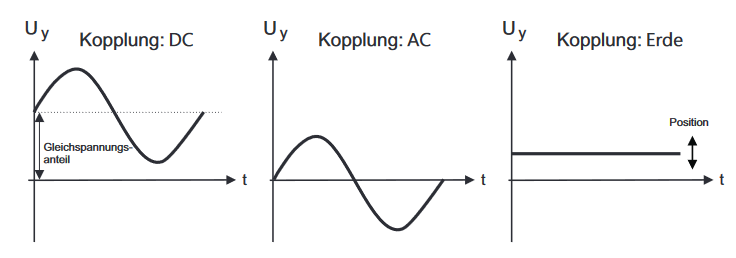
\includegraphics[width=9cm]{graphics/kopp.png}
    \caption{Sinussignal bei verschiedenen Kopplungen}
    \label{fig:kopp}
\end{figure}

\newpage

Zuletzt betrachten wir noch die zwei für diesen Versuch relevanten Physikalsischen Grundlagen.

Ein Aspekt hierbei ist die Pulsweitenmodulation. Sie dient der Dimmung einer LED, indem nicht die Amplitude der anliegenden Spannung reduziert wird, sondern die Spannung zwischendurch aus- und eingeschaltet wird. Dabei gibt das Verhältnis der Periodendauer $T$ zur Pulsdauer $t$ den Tastgrad, aus dem mit der Impulsspannung $U_0$ der Spannungsmittelwert $U_M$ und die effektive Spannung $U_{eff}$ bestimmt werden können:

\begin{equation}
    U_M = U_0 \frac{t}{T}
    \label{eq:Ummmm}
\end{equation}
\begin{equation}
    U_{eff} = U_0 \sqrt{\frac{t}{T}}
    \label{eq:Ufffff}
\end{equation}

Der zweite Aspekt ist die Reflexion auf einer Leitung. Trifft eine Welle von einem Medium auf ein Anderes so wird ein Anteil dieser Welle reflektiert. Dies geschieht auch bei elektromagnetischen Wellen in Abhängigkeit vom Wellenwiderstand des Materials, zum Beispiel des Kabels. Trifft eine elektromagnetische Welle von einem Material auf eine anderes mit unterschiedlichen Wellenwiderstand, so wird ein Teil des Signals reflektiert. Dies passiert vor allem am Ende von Kabeln. Der Wellenwiderstand $Z$ hängt dabei von der Induktivität des Materials pro Länge $L'$ und der Kapazität pro Länge $C'$ ab:

\begin{equation}
    Z = \sqrt{\frac{L'}{C'}}
\end{equation}

Die Refelxion am Kabelende kann umgangen werden, indem ein Widerstand gleich dem Wellenwiderstand des Kabels am Ende angebracht wird.

\subsection{Versuchsaufbau}

Eine Skizze des Aufbaus ist auf der nächsten Seite im Messprotokoll zu sehen. 

Bei diesem Versuch werden nacheinander verschiedene Signale an ein Oszilloskop angeschlossen. Zunächst betrachten wir ein einfaches Sinussignal von einem Funktionsgenerator. Anschließend nutzen wir den Signalgenerator, der eine Reihe unterschiedlicher Signale produzieren kann. Zum Schluss nutzen wir noch das zur Verfügung gestellte lange Koaxialkabel, um die Reflexion zu untersuchen.

%---------------VERSUCHSPROTOKOLL MIT MESSDATEN---------------
\newpage

\section{Versuchsprotokoll mit Messdaten}

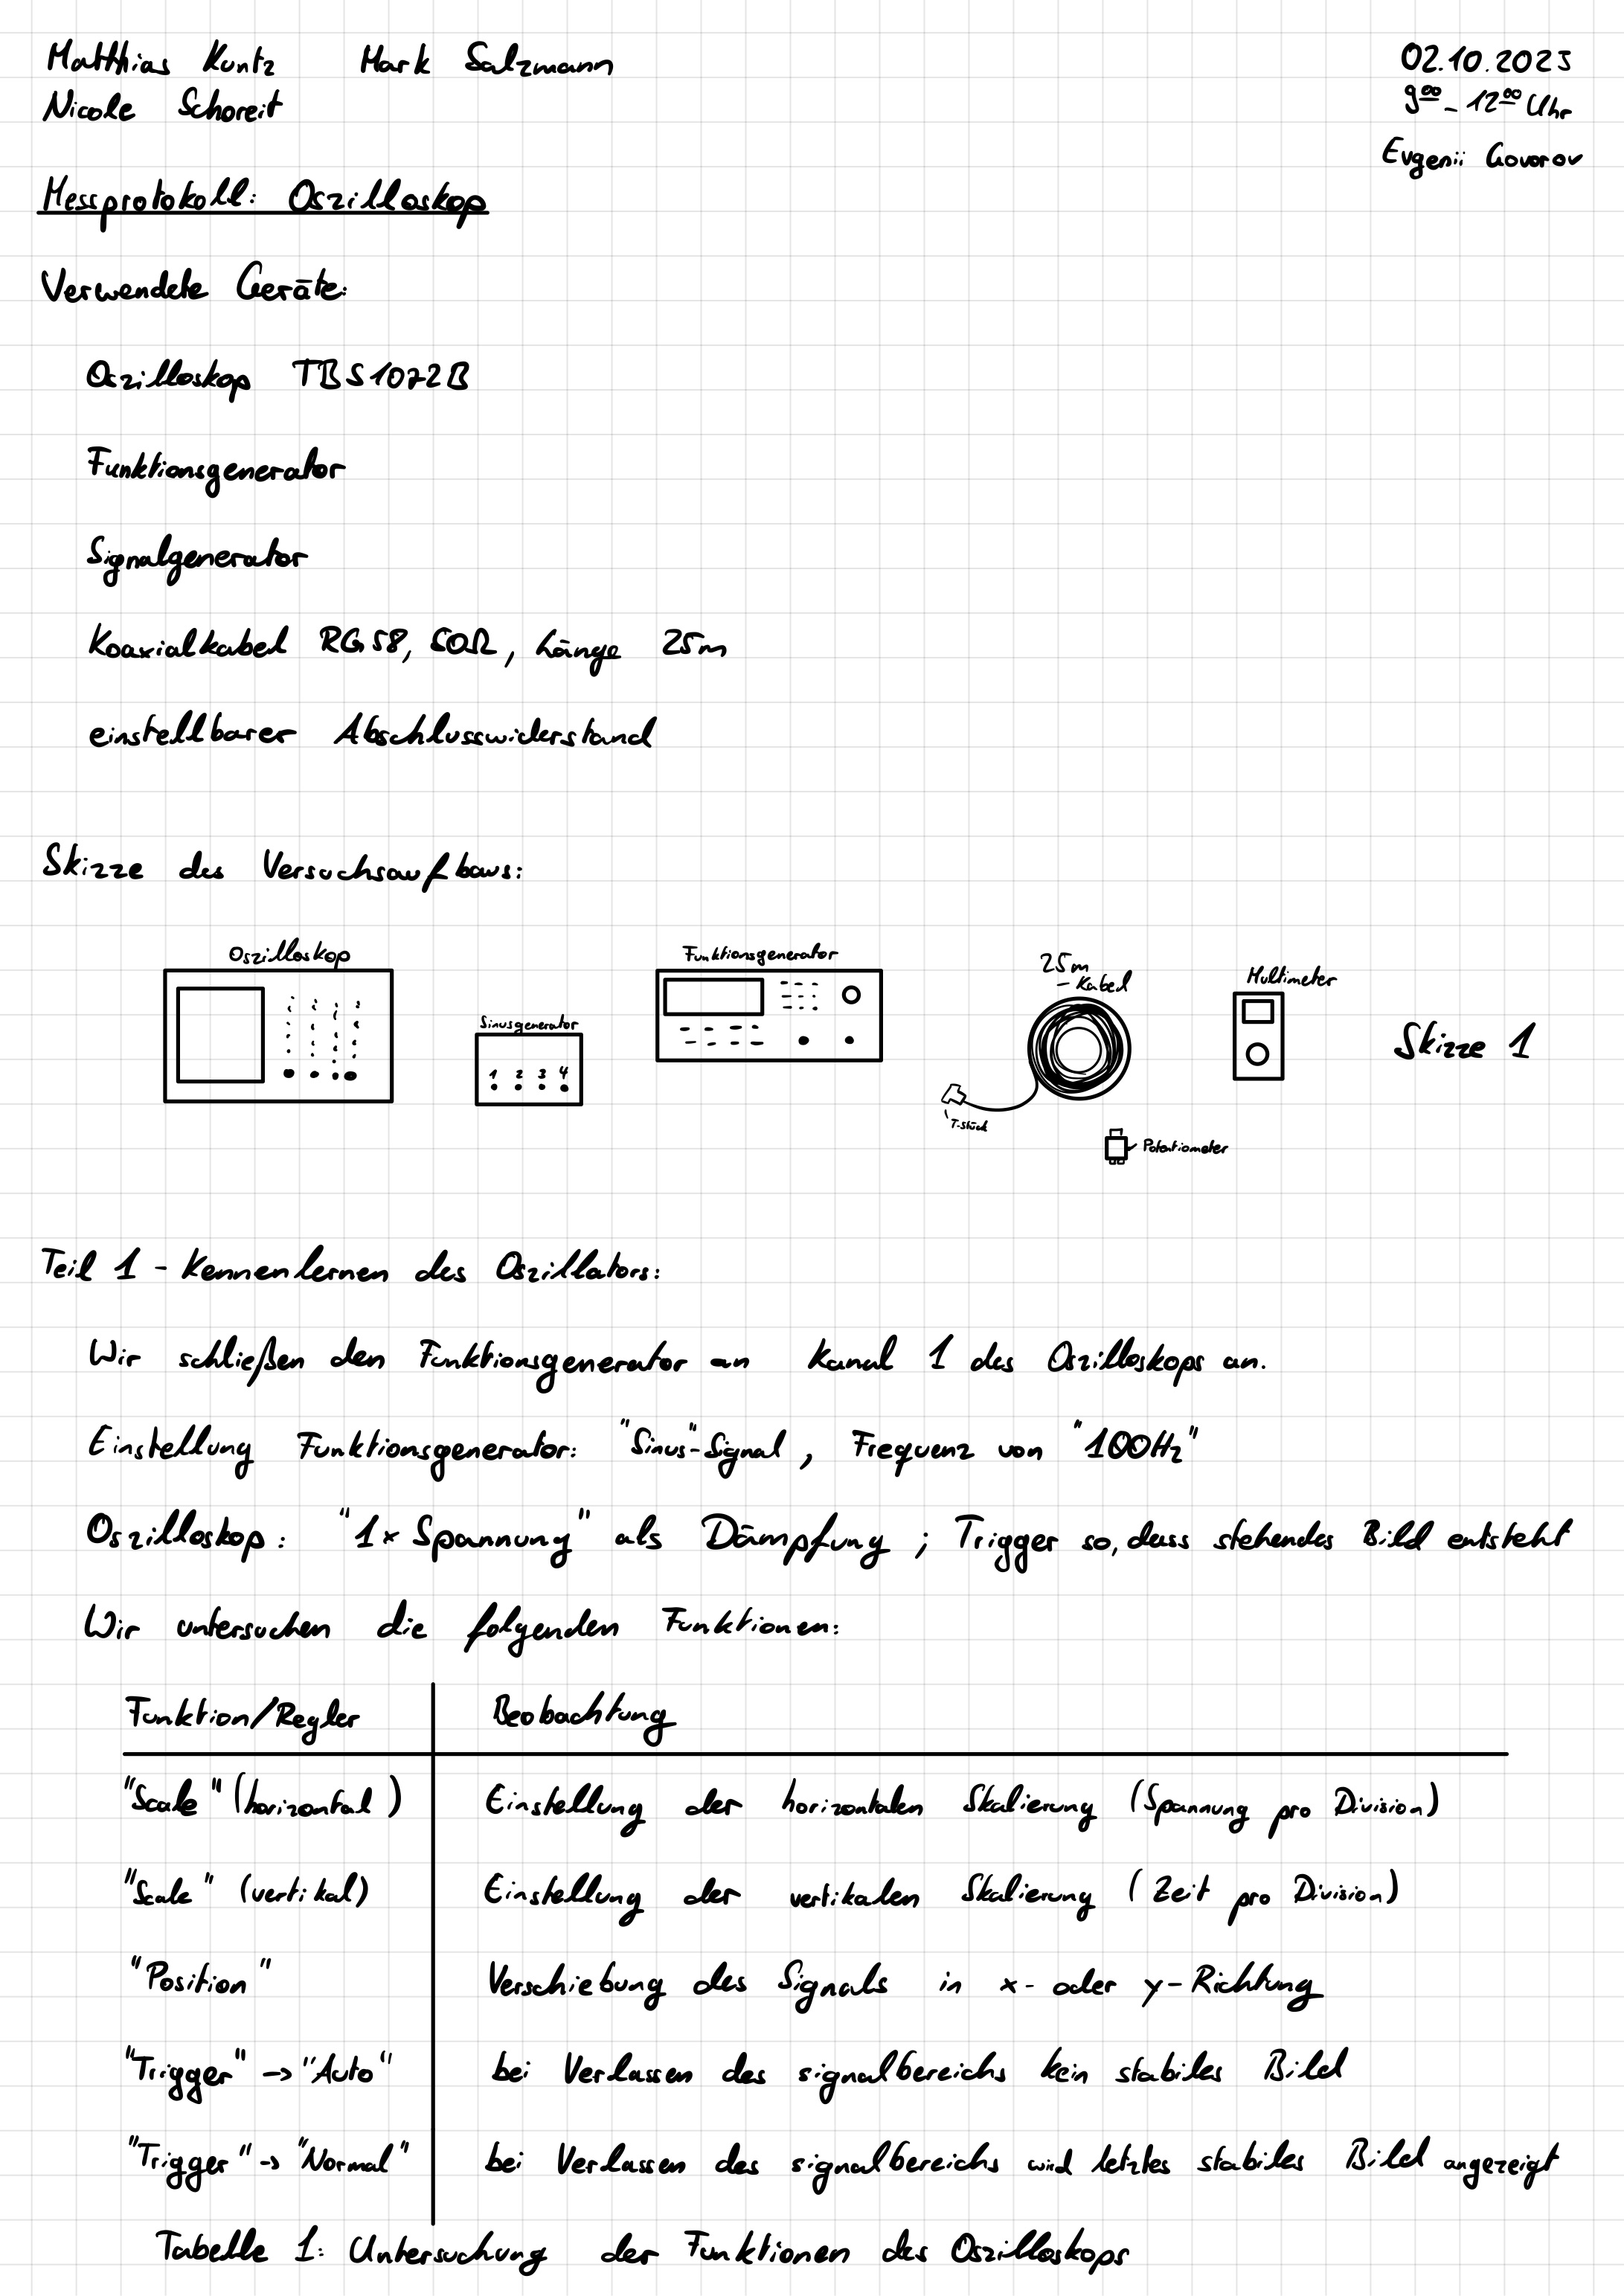
\includegraphics[width=\textwidth]{graphics/mess1.jpg}
\newpage
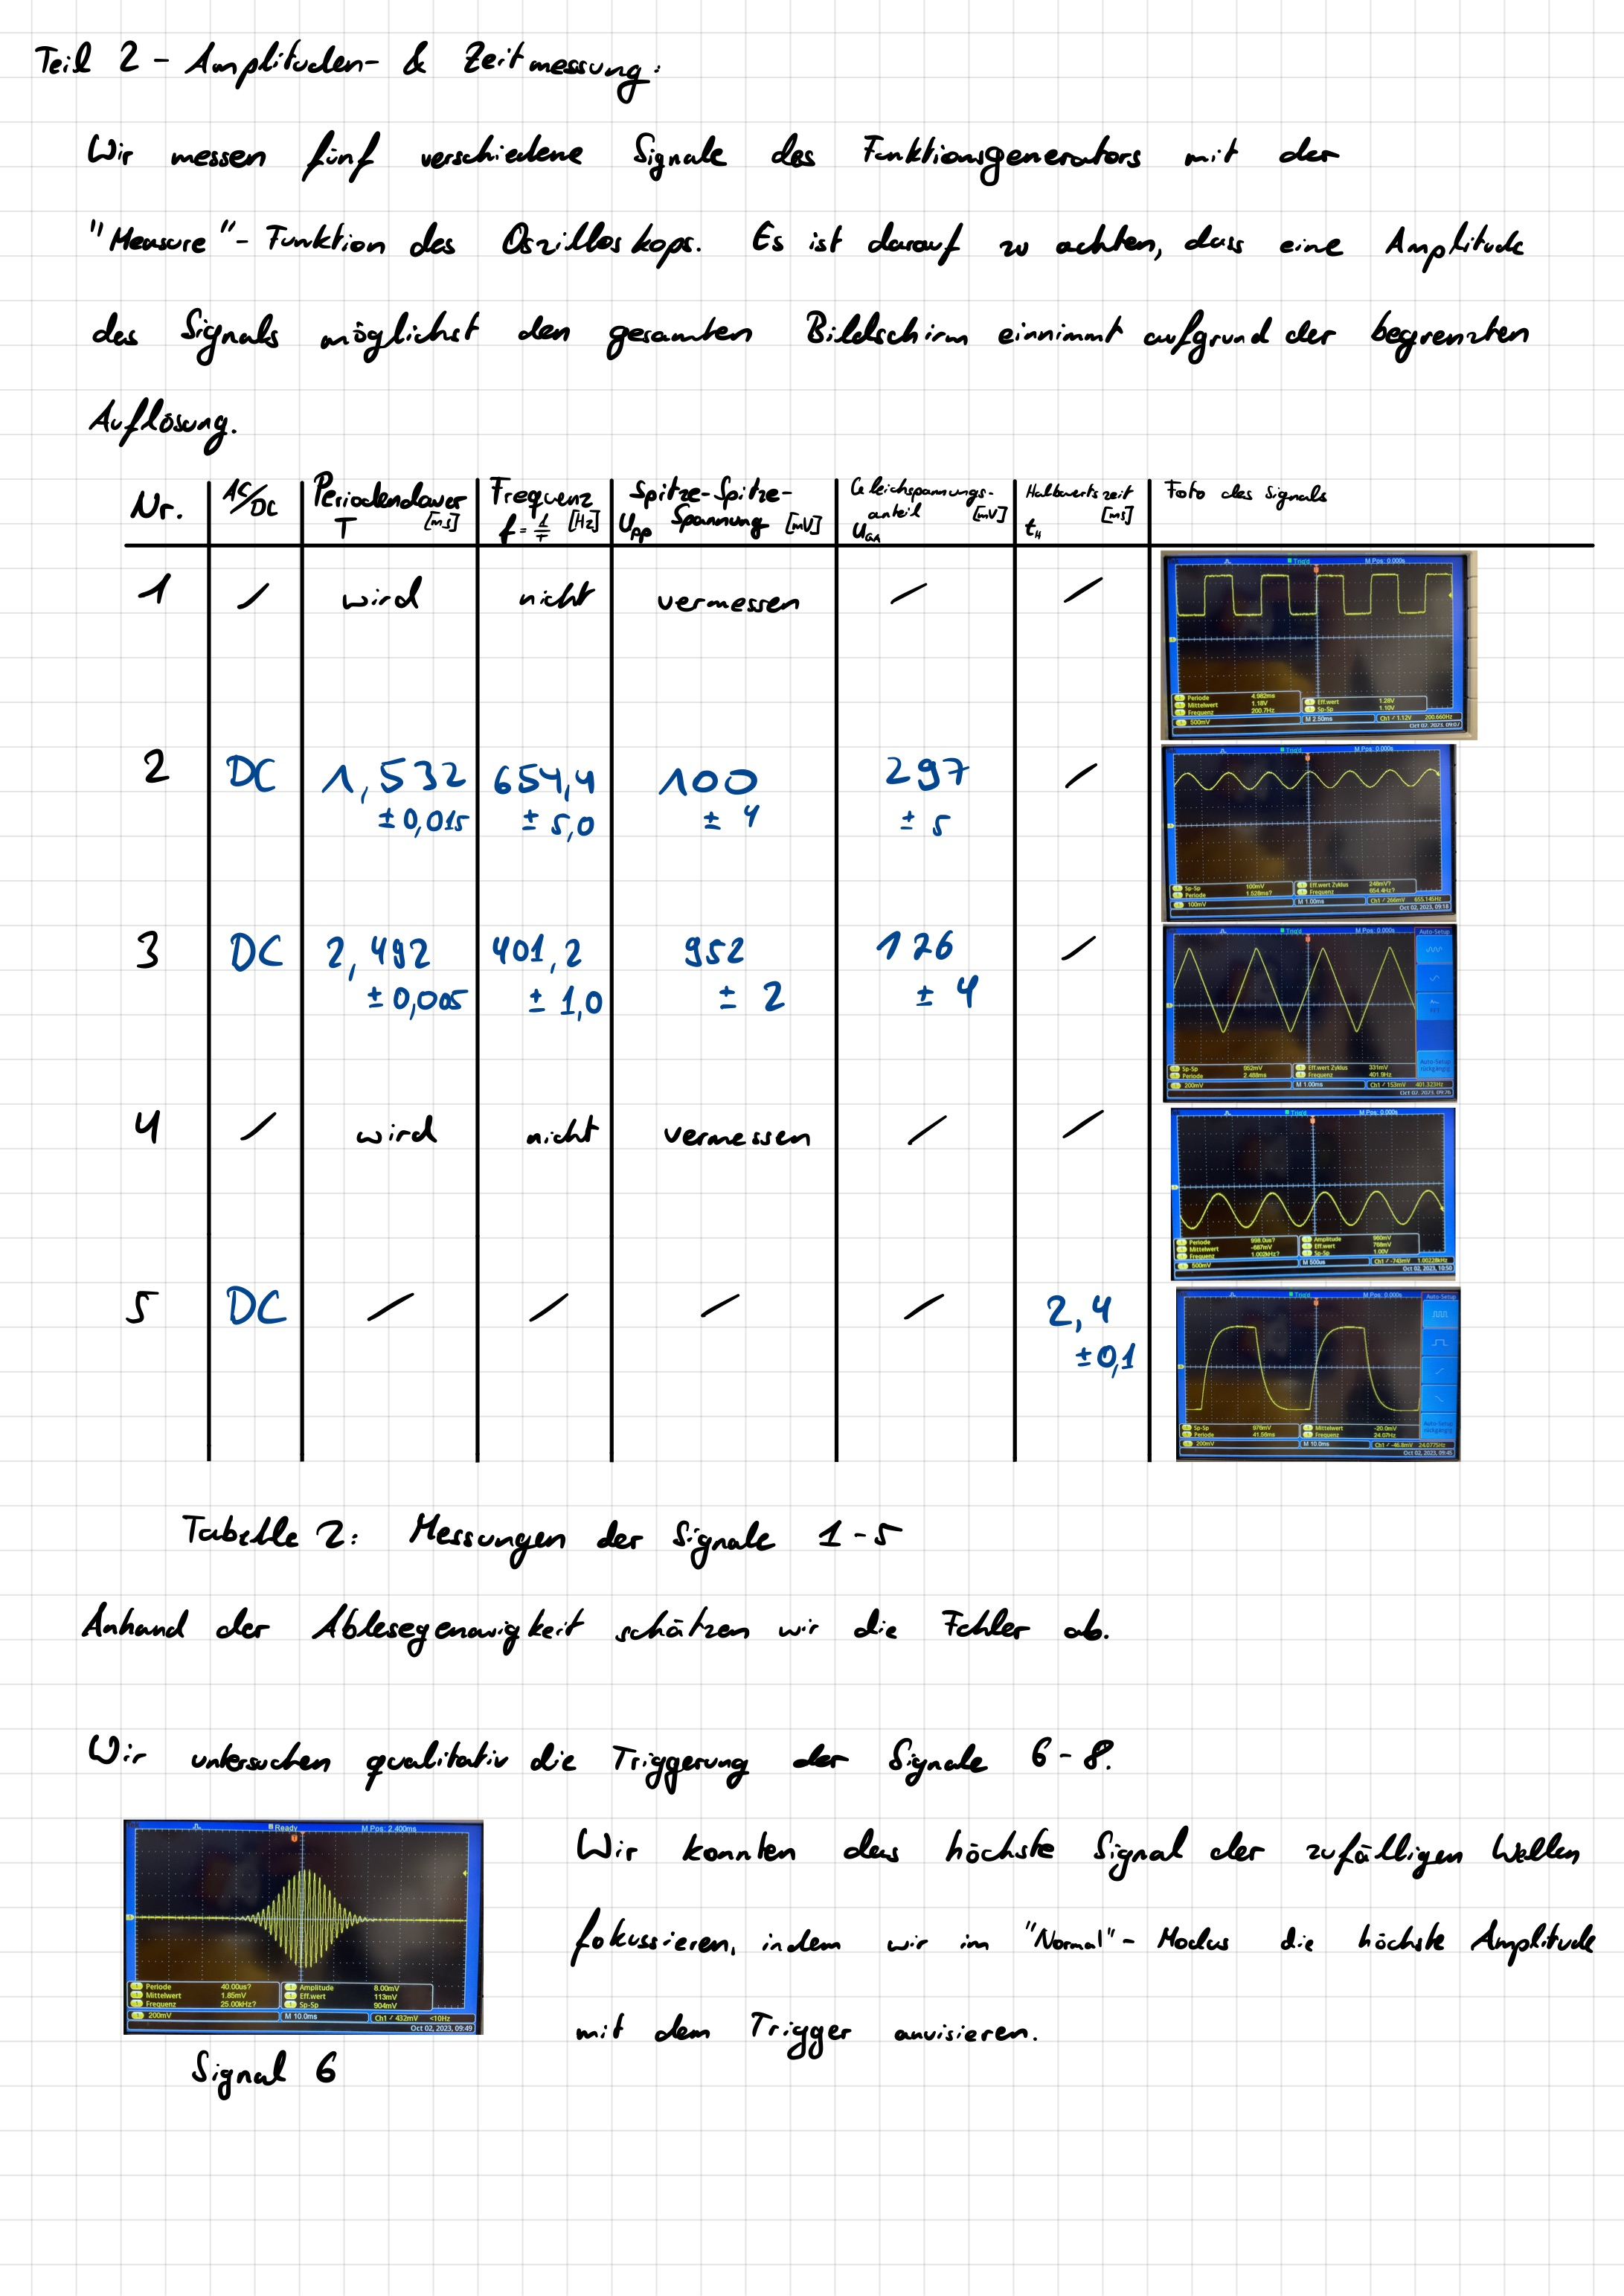
\includegraphics[width=\textwidth]{graphics/mess2.jpg}
\newpage
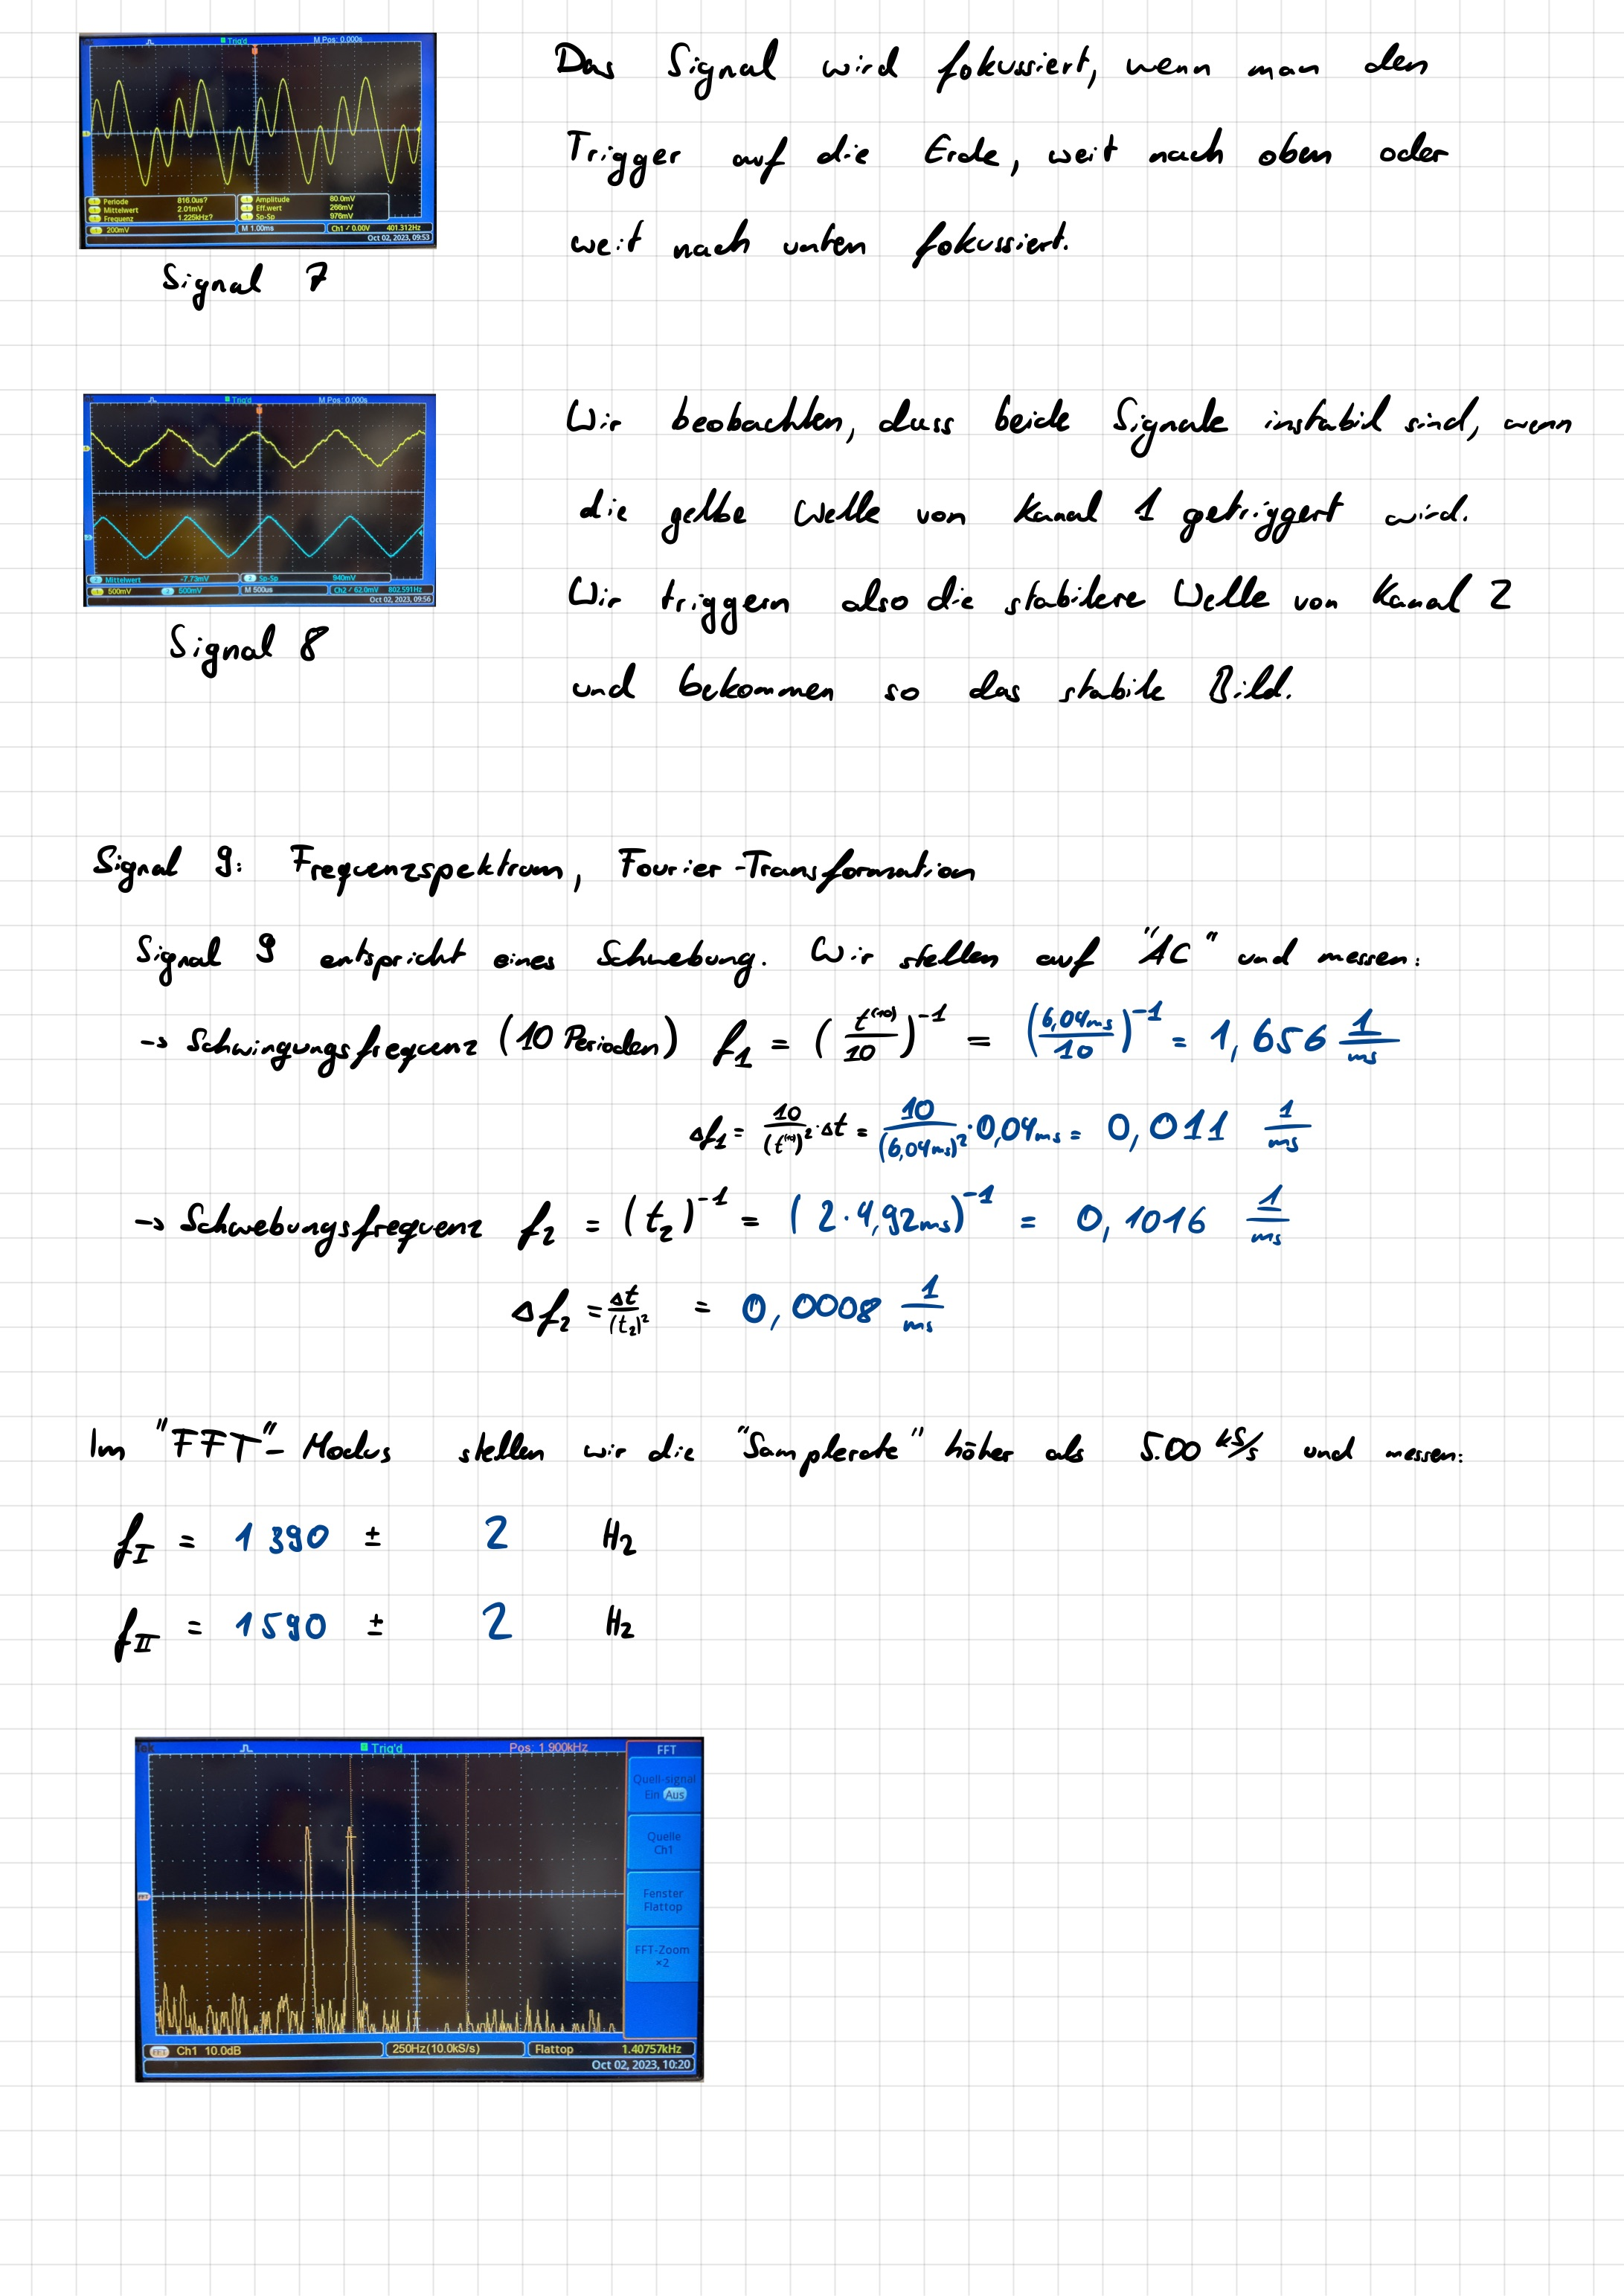
\includegraphics[width=\textwidth]{graphics/mess3.jpg}
\newpage
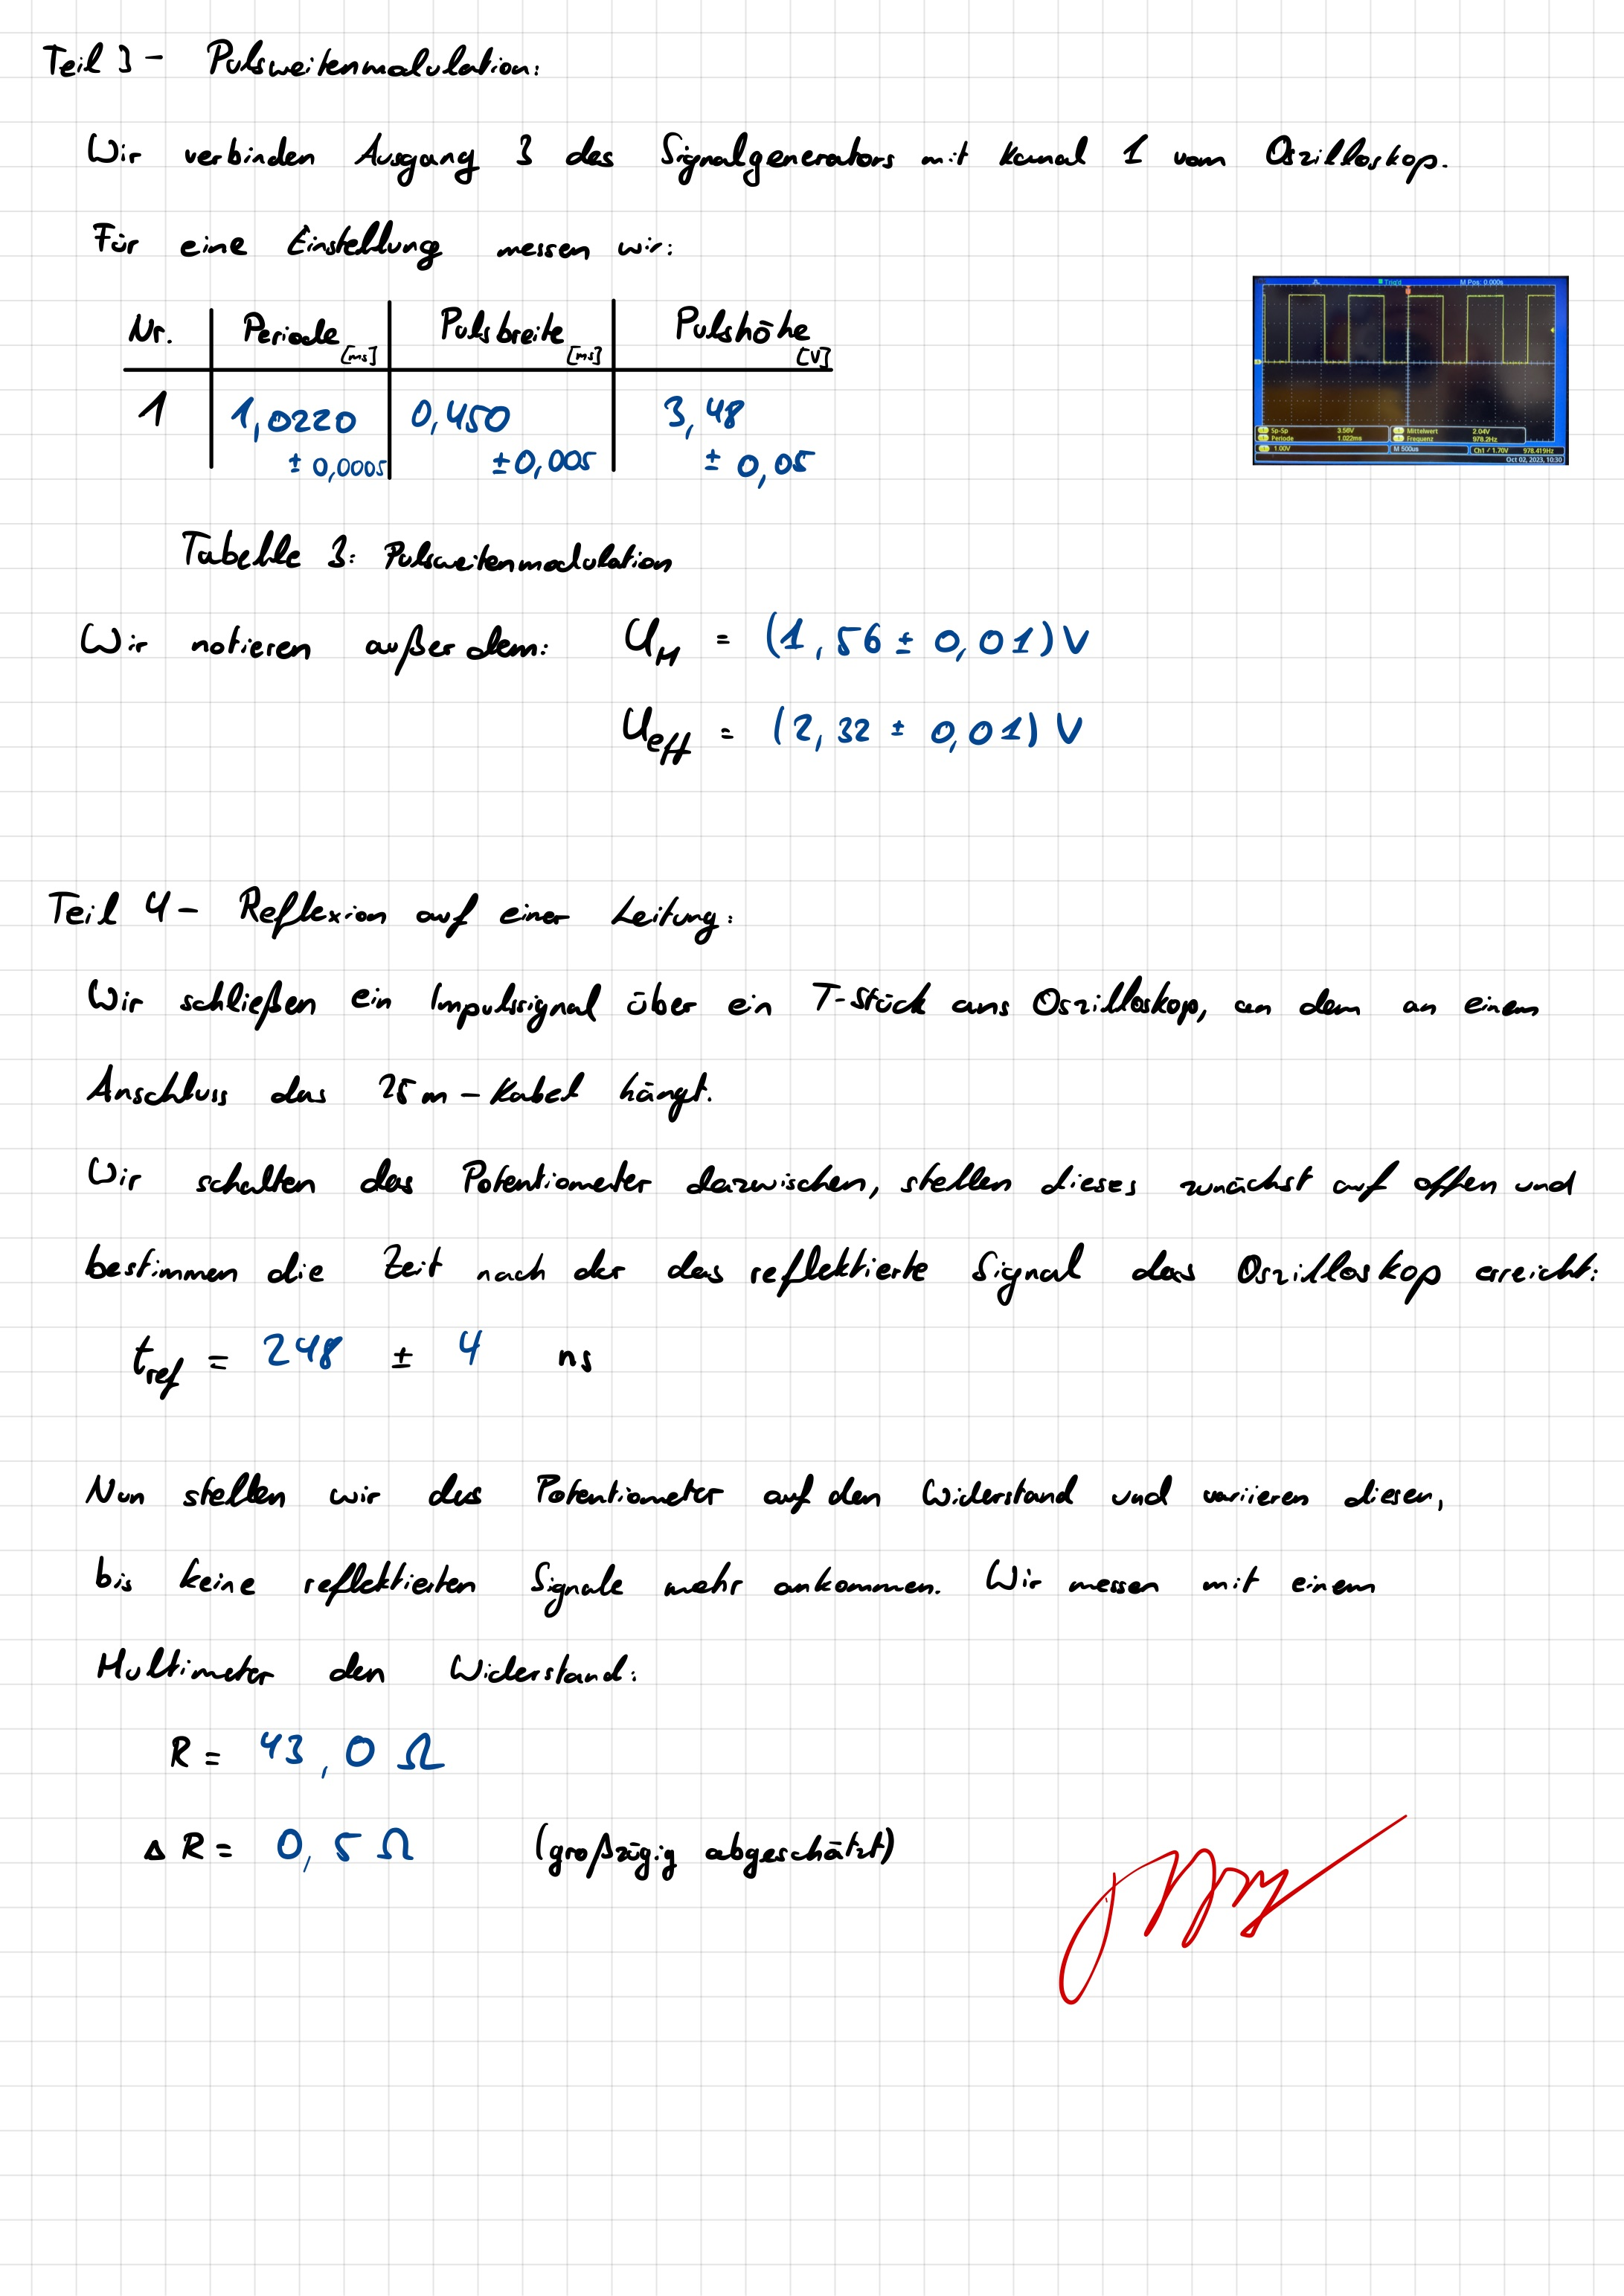
\includegraphics[width=\textwidth]{graphics/mess4.jpg}
\newpage

\addtocounter{table}{3}

%-------------------------AUSWERTUNG-------------------------
\section{Auswertung}

In dieser Evaluation werden alle Fehler, sofern keine spezifische Angabe gemacht wird, mithilfe der Gauss'schen Fehlerfortpflanzung berechnet. Dies bedeutet, dass ein Wert $F$, der mit der Formel $f(a_1, ..., a_n)$ berechnet wird, den Fehler $\Delta F$ gegeben über folgende Formel hat:

\begin{equation}
    \Delta F = \sqrt{\sum_n \left( \frac{\partial f}{\partial a_n} \cdot \Delta a_n \right)^2}.
\end{equation}

\subsection{Auswertung der vermessenen Signale}

Wir beginnen, indem wir die Messungen von Teil 2 in einer Tabelle eintragen und zu den beiden voll vermessenen Signalen 2 \& 3 noch die Maximal- $U_{max}$ und Minimalspannung $U_{min}$ berechnen:

\begin{equation}
    \begin{split}
        U_{max} &= U_{GA} + \frac{U_{SS}}{2}, \ \ \ \ U_{min} = U_{GA} - \frac{U_{SS}}{2} \\ \\
        \Delta U_{max} &= \Delta U_{min} = \sqrt{(\Delta U_{GA})^2 + \left( \frac{\Delta U_{SS}}{2} \right)^2}
    \end{split}
\end{equation}

Die Ergebnisse sind in Tabelle \ref{tab:smol} eingetragen.

\begin{table}[!ht]
\centering
\caption{Messergebnisse der Signale 2, 3 \& 5}
\centerline{
\resizebox{1.2\textwidth}{!}{
\begin{tabular}{c|c|c|c|c|c|c|c}
\hline
\textbf{Foto} & $\bm{T}$ [ms] & $\bm{f}$ [Hz] & $\bm{U_{SS}}$ [mV] & $\bm{U_{GA}}$ [mV] & $\bm{U_{max}}$ [mV] & $\bm{U_{min}}$ [mV] & $\bm{t_{\frac{1}{2}}}$ [ms] \\ \hline
    \rowincludegraphics[width=2cm]{graphics/sig2.jpg} & $1,532 \pm 0,015$ & $654 \pm 5$ & $100 \pm 4$ & $297 \pm 5$ & $347 \pm 5$ & $247 \pm 5$ & - \\
     & & & & & & & \\
    \rowincludegraphics[width=2cm]{graphics/sig3.jpg} & $2,492 \pm 0,0005$ & $401,2 \pm 1,0$ & $953 \pm 2$ & $176 \pm 4$ & $653 \pm 4$ & $-(301 \pm 4)$ & - \\
     & & & & & & & \\
    \rowincludegraphics[width=2cm]{graphics/sig5.jpg} &     -   &    -    &     -   &    -    &    -       &     -      & $2,40 \pm 0,10$ \\ \hline
\end{tabular}}}
\label{tab:smol}
\end{table}

\newpage

Zusätzlich werten wir die Messungen von Signal 9 im Fourier-Modus aus, indem wir manuell aus den gemessen Frequenzen der Peaks die Schwingungs- und Schwebefrequenzen $f'$ berechnen:

\begin{equation}
    \begin{split}
        f'_1 &= \frac{1}{2} (f_{II} + f_{I}), \ \ \ \ f'_2 = \frac{1}{2} (f_{II} - f_{I}) \\
        \Delta f'_1 &= \Delta f'_2 = \frac{1}{2} \sqrt{(\Delta f_{II})^2 + (\Delta f_{I})^2} \\ \\
        \implies \bm{f'_1} &= \bm{(1490,0 \pm 2,8)} \textbf{Hz} \\
        \bm{f'_2} &= \bm{(100 \pm 2,8)} \textbf{Hz}
    \end{split}
\end{equation}

Diese Werte können nun mit den manuell bestimmten Werten für die Schwebe- und Schwingfrequenz aus dem Messprotokoll verglichen werden. Wir verwenden dafür einen Signifikanztest:

\begin{equation}
    \begin{split}
        \sigma &= \frac{|f'-f|}{\sqrt{(\Delta f')^2 + (\Delta f)^2}} \\ \\
        \sigma_1 &= 14,62 \\
        \sigma_2 &= 0,55 \\
    \end{split}
\end{equation}

Die erste Abweichung ist mit einem Wert von 14,62 größer als der 3$\sigma$-Bereich und somit signifikant. Der zweite Wert ist insignifikant.

\newpage

\subsection{Pulsweitenmodulation}

Mit unseren Messungen aus Teil 3, Tabelle 3, bestimmen wir manuell mit den Gelichungen \ref{eq:Ummmm} \& \ref{eq:Ufffff} Mittelwert $U'_M$ und Effektivwert $U'_{eff}$:

\begin{equation}
    \begin{split}
        \Delta U'_M &= U'_M \sqrt{\left( \frac{\Delta t}{t} \right)^2 + \left( \frac{\Delta T}{T} \right)^2 + \left( \frac{\Delta U_0}{U_0} \right)^2} \\
        \Delta U'_{eff} &= U'_{eff} \sqrt{\left( \frac{\Delta t}{2t} \right)^2 + \left( \frac{\Delta T}{2T} \right)^2 + \left( \frac{\Delta U_0}{U_0} \right)^2} \\ \\
        \implies \bm{U'_M} &= \bm{(1,532 \pm 0,028)} \textbf{V} \\
        \bm{U'_{eff}} &= \bm{(2,31 \pm 0,04)} \textbf{V} \\
    \end{split}
\end{equation}

Wir vergleichen die berechneten Werte mit den gemessenen Werten aus dem Messprotokoll mithilfe des Signifikanztests:

\begin{equation}
    \begin{split}
        \sigma_M &= 0,94\\
        \sigma_{eff} &= 0,24 \\
    \end{split}
\end{equation}

Somit weisen beide Werte insignifikante Abweichungen auf.

\newpage

\subsection{Reflexion auf einer Leitung}

Aus der Laufzeit des Reflektierten Signals bestimmen wir die Länge des Kabels $l$. Dazu nehmen wir die Ausbreitungsgeschwindigkeit des Signals im Kabel als 66\% der Vakuumlichtgeschwindigkeit, wofür wir $c = 299792458$ m/s (Wikipedia, Stand: 03.10.2023) verwenden:

\begin{equation}
    \begin{split}
        l = 0,66 c \cdot \frac{1}{2} & t_{ref}, \ \  \ \ \Delta l = 0,66 c \cdot \frac{1}{2} \Delta t_{ref} \\ \\
        \implies \bm{l} &= \bm{(24,5 \pm 0,4) \frac{\textbf{m}}{\textbf{s}}}  
    \end{split}
\end{equation}

Verglichen mit der angegeben Länge von 25m ergibt sich eine insignifikante Abweichung von $\sigma = 1,25$.

Wir wollen zuletzt den gemessenen Widerstand R=$(43,0 \pm 0,5) \Omega$ mit dem Wellenwiderstand des Kabels vergleichen. Dazu entnehmen wir diesen als 50$\Omega$ aus dem Kabeltyp RG58. Wir erhalten $\sigma = 14$, was eine signifikante Abweichung darstellt.

\newpage
%---------------ZUSAMMENFASSUNG UND DISKUSSION---------------
\section{Zusammenfassung und Diskussion}

In diesem Versuch haben wir mit verschiedenen Messungen unterschiedlicher Signale die Funktionen und Bedienung eines Oszilloskops kennengelernt. Eingeführt wurde die grundlegenden Einstellungen und Anzeigen sowie Tools wie die Curser- und Measure-Funktionen. Auch haben wir den FFT-Modus mit den Fourier-transformierten Signalen bei der Schwebung sowie die Reflexion auf einer Leitung beobachtet. 

Die Ergebnisse der Auswertung wiesen teils große Sigmaabweichungen auf. Grund hierfür wird vorüberwiegend eine nicht ausreichend große Abschätzung der Fehler gewesen sein. Insbesondere beim letzten Versuchsteil, in dem mithilfe eines Drehknopfs der Widerstand am Kabelende variiert werden musste, war die Einstellung sehr ungenau und es war nicht gut abzuschätzen, wann genau kein reflektiertes Signal mehr beim Oszilloskop ankam. Im Zuge dessen wird der gewählte Fehler von 0,5$\Omega$ zu klein gewählt sein. Analog wird bei der Untersuchung der Schwebung der Fehler der Frequenzen im FFT-Modus zu klein abgeschätzt worden sein. Hier war bei der Durchführung die Auflösung des Oszilloskops ein Hindernis, dessen Einfluss auf den finalen Wert wohl zu sehr unterschätzt wurde.

Abgesehen davon lagen alle anderen Werte in erwarteten Bereichen und insignifikanten Abweichungen. 

Somit lässt sich final das Fazit ziehen, dass dieser Versuch eine gute Einführung in eine große Anzahl an Funktionen des Oszilloskops lieferte. Da die bestimmten Werte auch nicht allgemeine Konstanten oder andere Werte waren, die mit Literaturwerten hätten verglichen werden müssen, mit Außnahme vom Widerstand im letzten Teil, war auch der Druck ein 100\% richtiges Ergebnis zu erzielen genommen und die Funktionsweise sowie der Umgang mit dem Oszilloskop standen im Vordergrund. Die hohen Sigmawerte sind natürlich dennoch ärgerlich, lassen sich aber auf eine anfängliche Unvertrautheit mit dem Gerät zurückführen und dienen somit als Warnhinweise für zukünftige Experimente mit Oszilloskopen. 

\end{document}

